% Options for packages loaded elsewhere
\PassOptionsToPackage{unicode}{hyperref}
\PassOptionsToPackage{hyphens}{url}
\PassOptionsToPackage{dvipsnames,svgnames,x11names}{xcolor}
%
\documentclass[
  letterpaper,
  DIV=11,
  numbers=noendperiod]{scrartcl}

\usepackage{amsmath,amssymb}
\usepackage{lmodern}
\usepackage{iftex}
\ifPDFTeX
  \usepackage[T1]{fontenc}
  \usepackage[utf8]{inputenc}
  \usepackage{textcomp} % provide euro and other symbols
\else % if luatex or xetex
  \usepackage{unicode-math}
  \defaultfontfeatures{Scale=MatchLowercase}
  \defaultfontfeatures[\rmfamily]{Ligatures=TeX,Scale=1}
\fi
% Use upquote if available, for straight quotes in verbatim environments
\IfFileExists{upquote.sty}{\usepackage{upquote}}{}
\IfFileExists{microtype.sty}{% use microtype if available
  \usepackage[]{microtype}
  \UseMicrotypeSet[protrusion]{basicmath} % disable protrusion for tt fonts
}{}
\makeatletter
\@ifundefined{KOMAClassName}{% if non-KOMA class
  \IfFileExists{parskip.sty}{%
    \usepackage{parskip}
  }{% else
    \setlength{\parindent}{0pt}
    \setlength{\parskip}{6pt plus 2pt minus 1pt}}
}{% if KOMA class
  \KOMAoptions{parskip=half}}
\makeatother
\usepackage{xcolor}
\setlength{\emergencystretch}{3em} % prevent overfull lines
\setcounter{secnumdepth}{-\maxdimen} % remove section numbering
% Make \paragraph and \subparagraph free-standing
\ifx\paragraph\undefined\else
  \let\oldparagraph\paragraph
  \renewcommand{\paragraph}[1]{\oldparagraph{#1}\mbox{}}
\fi
\ifx\subparagraph\undefined\else
  \let\oldsubparagraph\subparagraph
  \renewcommand{\subparagraph}[1]{\oldsubparagraph{#1}\mbox{}}
\fi


\providecommand{\tightlist}{%
  \setlength{\itemsep}{0pt}\setlength{\parskip}{0pt}}\usepackage{longtable,booktabs,array}
\usepackage{calc} % for calculating minipage widths
% Correct order of tables after \paragraph or \subparagraph
\usepackage{etoolbox}
\makeatletter
\patchcmd\longtable{\par}{\if@noskipsec\mbox{}\fi\par}{}{}
\makeatother
% Allow footnotes in longtable head/foot
\IfFileExists{footnotehyper.sty}{\usepackage{footnotehyper}}{\usepackage{footnote}}
\makesavenoteenv{longtable}
\usepackage{graphicx}
\makeatletter
\def\maxwidth{\ifdim\Gin@nat@width>\linewidth\linewidth\else\Gin@nat@width\fi}
\def\maxheight{\ifdim\Gin@nat@height>\textheight\textheight\else\Gin@nat@height\fi}
\makeatother
% Scale images if necessary, so that they will not overflow the page
% margins by default, and it is still possible to overwrite the defaults
% using explicit options in \includegraphics[width, height, ...]{}
\setkeys{Gin}{width=\maxwidth,height=\maxheight,keepaspectratio}
% Set default figure placement to htbp
\makeatletter
\def\fps@figure{htbp}
\makeatother

\KOMAoption{captions}{tableheading}
\makeatletter
\makeatother
\makeatletter
\@ifpackageloaded{caption}{}{\usepackage{caption}}
\AtBeginDocument{%
\ifdefined\contentsname
  \renewcommand*\contentsname{Table of contents}
\else
  \newcommand\contentsname{Table of contents}
\fi
\ifdefined\listfigurename
  \renewcommand*\listfigurename{List of Figures}
\else
  \newcommand\listfigurename{List of Figures}
\fi
\ifdefined\listtablename
  \renewcommand*\listtablename{List of Tables}
\else
  \newcommand\listtablename{List of Tables}
\fi
\ifdefined\figurename
  \renewcommand*\figurename{Figure}
\else
  \newcommand\figurename{Figure}
\fi
\ifdefined\tablename
  \renewcommand*\tablename{Table}
\else
  \newcommand\tablename{Table}
\fi
}
\@ifpackageloaded{float}{}{\usepackage{float}}
\floatstyle{ruled}
\@ifundefined{c@chapter}{\newfloat{codelisting}{h}{lop}}{\newfloat{codelisting}{h}{lop}[chapter]}
\floatname{codelisting}{Listing}
\newcommand*\listoflistings{\listof{codelisting}{List of Listings}}
\makeatother
\makeatletter
\@ifpackageloaded{caption}{}{\usepackage{caption}}
\@ifpackageloaded{subcaption}{}{\usepackage{subcaption}}
\makeatother
\makeatletter
\@ifpackageloaded{tcolorbox}{}{\usepackage[many]{tcolorbox}}
\makeatother
\makeatletter
\@ifundefined{shadecolor}{\definecolor{shadecolor}{rgb}{.97, .97, .97}}
\makeatother
\makeatletter
\makeatother
\ifLuaTeX
  \usepackage{selnolig}  % disable illegal ligatures
\fi
\usepackage[]{biblatex}
\addbibresource{Prueba.bib}
\IfFileExists{bookmark.sty}{\usepackage{bookmark}}{\usepackage{hyperref}}
\IfFileExists{xurl.sty}{\usepackage{xurl}}{} % add URL line breaks if available
\urlstyle{same} % disable monospaced font for URLs
\hypersetup{
  pdftitle={Taller 0: Herramientas de Organización en PyMES y Micro Pymes.},
  colorlinks=true,
  linkcolor={blue},
  filecolor={Maroon},
  citecolor={Blue},
  urlcolor={Blue},
  pdfcreator={LaTeX via pandoc}}

\title{Taller 0: Herramientas de Organización en PyMES y Micro Pymes.}
\author{}
\date{5/24/22}

\begin{document}
\maketitle
\ifdefined\Shaded\renewenvironment{Shaded}{\begin{tcolorbox}[interior hidden, sharp corners, enhanced, frame hidden, breakable, boxrule=0pt, borderline west={3pt}{0pt}{shadecolor}]}{\end{tcolorbox}}\fi

\hypertarget{herramientas-de-organizaciuxf3n-para-pymes-y-micro-pymes.}{%
\section{Herramientas de Organización para Pymes y Micro
Pymes.}\label{herramientas-de-organizaciuxf3n-para-pymes-y-micro-pymes.}}

\textbf{Autor:} Lic. Diego Saavedra Mg. Sc.

\textbf{Institución:} Instituto Superior Tecnológico Juan Montalvo.

\hypertarget{herramientas-de-organizaciuxf3n-en-pymes-y-micro-pymes.}{%
\subsection{Herramientas de Organización en PyMES y Micro
Pymes.}\label{herramientas-de-organizaciuxf3n-en-pymes-y-micro-pymes.}}

\begin{figure}

{\centering 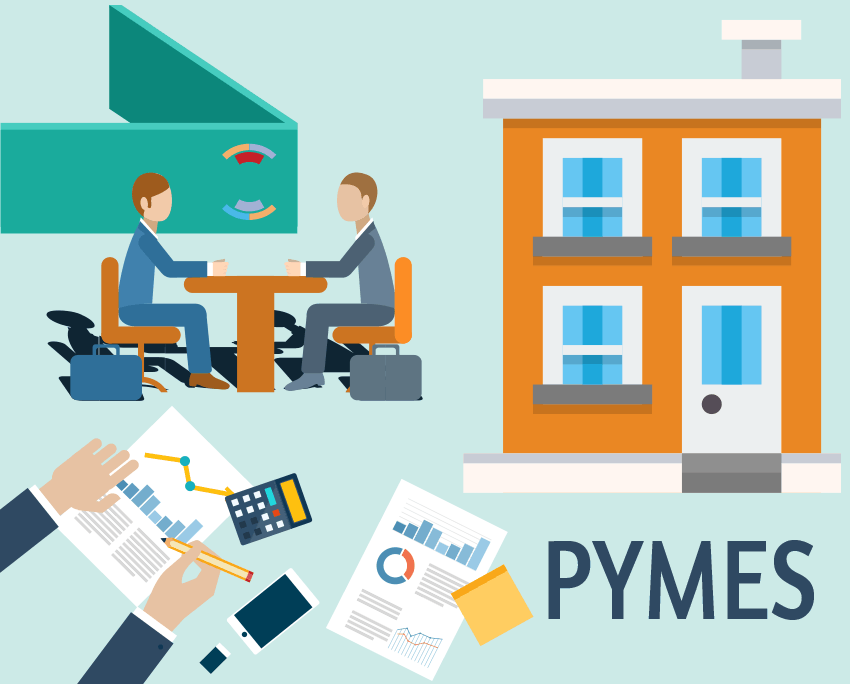
\includegraphics{media/pymes-babos.png}

}

\caption{PyMES y Micro Pymes}

\end{figure}

\hypertarget{herramientas-de-organizaciuxf3n-en-pymes-y-micro-pymes.-1}{%
\subsection{Herramientas de Organización en PyMES y Micro
Pymes.}\label{herramientas-de-organizaciuxf3n-en-pymes-y-micro-pymes.-1}}

Según \textcite{pregoWhatsAppAbreSu2022} la app de mensajería dispone ya
desde hace tiempo de un servicio pensado para la comunicación
empresarial, WhatsApp Business, y una plataforma de negocios que
---entre otras cosas--- permite generar un sistema de respuestas
automáticas, bots, para facilitar el contacto entre los negocios y sus
clientes.

Por otra parte se anuncia la apertura de una API que beneficiará a
importantes PyMES y Micro Pymes \textcite{pregoWhatsAppAbreSu2022}.

\hypertarget{herramientas-de-organizaciuxf3n-en-pymes-y-micro-pymes.-2}{%
\subsection{Herramientas de Organización en PyMES y Micro
Pymes.}\label{herramientas-de-organizaciuxf3n-en-pymes-y-micro-pymes.-2}}

Por otra parte \textcite{rodriguezAmazonOfreceGratuitamente2021} la
oferta de Amazon incluye 50 escritorios en remoto, un paquete de
rendimiento de Windows, dos paquetes estándar de Linux y un paquete de
valor de Windows de Workspaces, que podrán usarla sin cargos hasta el 31
de julio de 2021.

La compañía de Jeff Bezos ya había ofrecido estos servicios de forma
gratuita hasta julio de 2020, tras la declaración de la pandemia mundial
de coronavirus y la migración masiva al teletrabajo como consecuencia de
ésta.

\hypertarget{workspaces-google.}{%
\subsection{Workspaces Google.}\label{workspaces-google.}}

\begin{longtable}[]{@{}
  >{\raggedright\arraybackslash}p{(\columnwidth - 2\tabcolsep) * \real{0.4545}}
  >{\raggedleft\arraybackslash}p{(\columnwidth - 2\tabcolsep) * \real{0.5455}}@{}}
\caption{Herramientas en PyMES y Micro Pymes.}\tabularnewline
\toprule()
\begin{minipage}[b]{\linewidth}\raggedright
Workspaces Google
\end{minipage} & \begin{minipage}[b]{\linewidth}\raggedleft
Herramientas
\end{minipage} \\
\midrule()
\endfirsthead
\toprule()
\begin{minipage}[b]{\linewidth}\raggedright
Workspaces Google
\end{minipage} & \begin{minipage}[b]{\linewidth}\raggedleft
Herramientas
\end{minipage} \\
\midrule()
\endhead
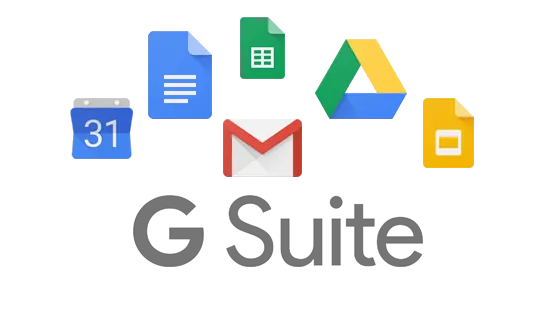
\includegraphics{media/gsuite.png} & 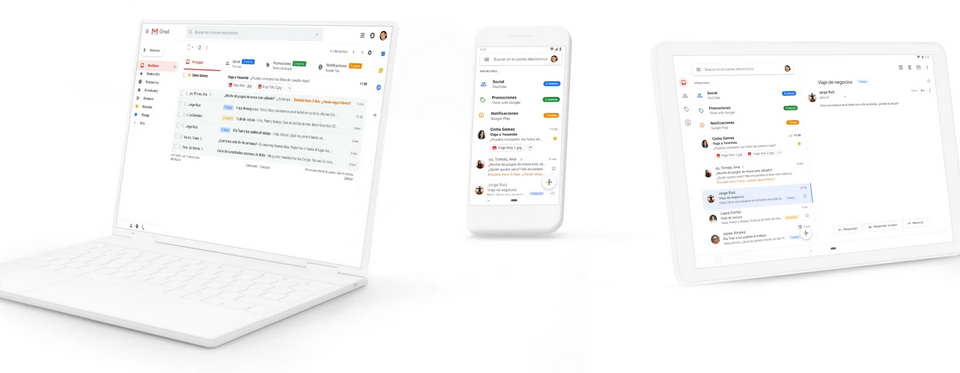
\includegraphics{media/pcs.png} \\
\bottomrule()
\end{longtable}

\hypertarget{workspaces-google.-1}{%
\subsection{Workspaces Google.}\label{workspaces-google.-1}}

Durante la pandemia aparecieron soluciones como \textbf{Google For
Educsation} para que niños y jovenes se puedan educar de forma
\textbf{gratuita} de acuerdo a la página oficial
\textcite{SolucionesDisenadasPara2022} esto permitió a profesores de
distintas instituciones educativas poder utilizar diferentes
herramientas de \textbf{Google} como Drive, Meet, Gmail, entre otros
(Servicios propios de G Suite ahora llamado Workspaces).

\hypertarget{calendario-sincronizado-en-la-organizaciuxf3n.}{%
\subsection{Calendario sincronizado en la
organización.}\label{calendario-sincronizado-en-la-organizaciuxf3n.}}

\begin{figure}

{\centering 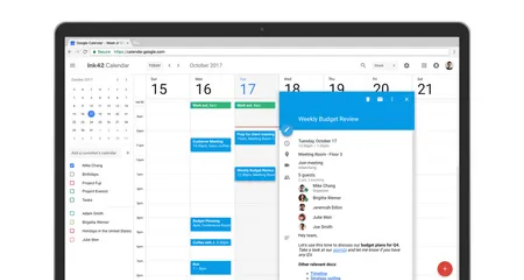
\includegraphics{media/calendario.png}

}

\caption{Calendario}

\end{figure}

\hypertarget{calendario-sincronizado-en-la-organizaciuxf3n.-1}{%
\subsection{Calendario sincronizado en la
organización.}\label{calendario-sincronizado-en-la-organizaciuxf3n.-1}}

Workspace Calendar permite sincronizar eventos, recordatorios o
reuniones de forma gratuita para Pymes y Micro Pymes de forma gratuita,
además de configurar de forma sencilla y agregando reuniones de Meet,
Zoom, entre otras herramientas
\textcite{CalendarioGoogleCalendarios2022}.

\hypertarget{conversaciones-seguras-y-centralizadas-con-el-chat}{%
\subsection{Conversaciones seguras y centralizadas con el
chat}\label{conversaciones-seguras-y-centralizadas-con-el-chat}}

\begin{figure}

{\centering 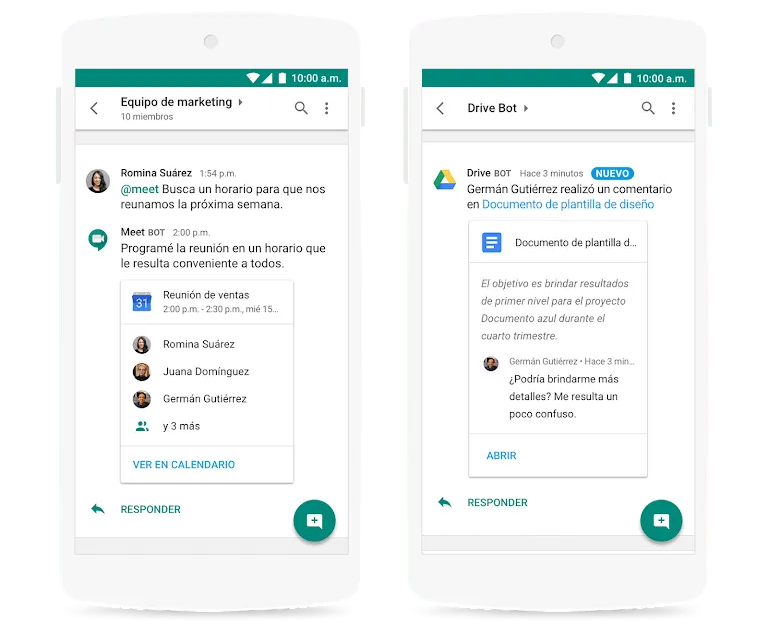
\includegraphics{media/conversaciones.png}

}

\caption{Conversaciones Seguras}

\end{figure}

\hypertarget{conversaciones-seguras-y-centralizadas-con-el-chat-1}{%
\subsection{Conversaciones seguras y centralizadas con el
chat}\label{conversaciones-seguras-y-centralizadas-con-el-chat-1}}

Preguntas como ¿dónde esta el servidor? ¿quién lo administra?¿en qué
país y bajo que legislación estarán protegidos mis datos? son las que se
hace \textcite{NextcloudOnlyOfficeRafael2020} en su artículo ``Nextcloud
+ OnlyOffice'', de lo cual se puede conocer que las conversaciones no
son seguras y existen herramientas de software libre que nos permiten
mejorar las propuestas de segurdiad en las Pymes y Micro Pymes.

\hypertarget{drive-para-documentos-en-la-nube}{%
\subsection{Drive para Documentos en la
nube}\label{drive-para-documentos-en-la-nube}}

\begin{figure}

{\centering 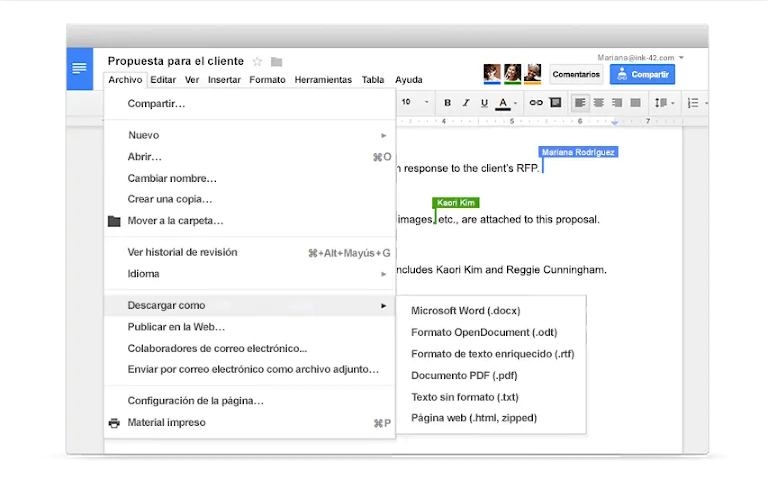
\includegraphics{media/drive.png}

}

\caption{Workspaces Drive}

\end{figure}

\hypertarget{drive-para-documentos-en-la-nube-1}{%
\subsection{Drive para Documentos en la
nube}\label{drive-para-documentos-en-la-nube-1}}

Existen varias nubes existentes en la actualidad,
\textcite{martiGoogleDriveVs2021} analiza \textbf{Dropbox, OneDrive,
Google Drive y iCloud,}. Estos servicios permiten a las PyMES y Micro
Pymes poder almacenar sus archivos en espacios fuera de la organización,
se recomienda revisar alternativas como las que menciona en su artículo
\textcite{RafaelBonifazSoftware2020} para tener más control de la
información privada.

\hypertarget{todo-en-mobile.}{%
\subsection{Todo en Mobile.}\label{todo-en-mobile.}}

\begin{figure}

{\centering 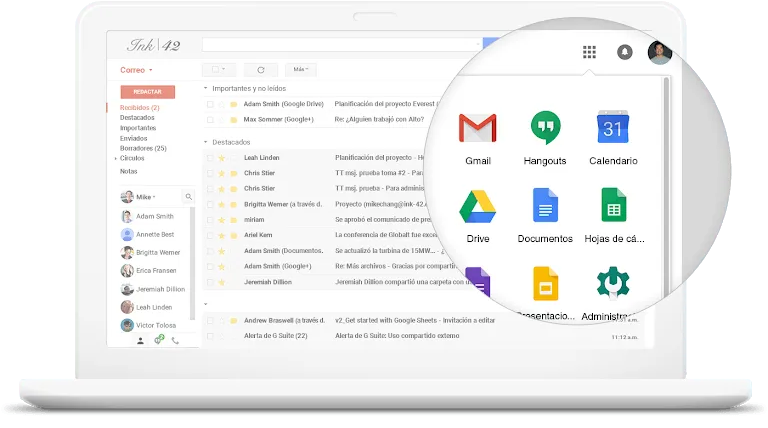
\includegraphics{media/mobile.png}

}

\caption{Mobile}

\end{figure}

\hypertarget{todo-en-mobile.-1}{%
\subsection{Todo en Mobile.}\label{todo-en-mobile.-1}}

Google anuncio en 200 ``Workspace'', su nueva plataforma de colaboración
para pequeñas y grandes empresas que viene a sustituir y unificar G
Suite. Se trata de un espacio de trabajo para usuarios profesionales que
integra todos los servicios de Google, a saber Gmail, Calendar, Drive,
Docs y Meet. De esa forma, los trabajadores y usuarios pueden acceder a
todo tipo de documentos o contenidos desde un mismo lugar según
\textcite{garciaSuiteAhoraEs2020}.

\hypertarget{propuesta}{%
\section{Propuesta}\label{propuesta}}

\begin{itemize}
\tightlist
\item
  Curso de G Suite (Documents, Shets, Presentations, Calendar, etc.).
\item
  Curso de Comunicaciones Seguras.
\item
  Uso adecuado del móvil.
\end{itemize}

\hypertarget{referencias}{%
\subsection{Referencias}\label{referencias}}


\printbibliography


\end{document}
